% ====================================================================
%+
% SECTION:
%    SolarSystem_AsteroidLightCurves.tex
%
% CHAPTER:
%    solarsystem.tex
%
% ELEVATOR PITCH:
%-
% ====================================================================

\section{Measuring Asteroid Light Curves and Rotation Periods}
\def\secname{\chpname:lightcurves}\label{sec:\secname}

\credit{rhiannonlynne},
\credit{davidtrilling}

Two Solar System science projects require a series of photometric
measurements. These are (1) measuring lightcurves and therefore shapes
of minor bodies and (2) measuring the colors and therefore compositions
of minor bodies. This section and the next describe the science and the
metrics for these experiments.

% --------------------------------------------------------------------

\subsection{Target measurements and discoveries}
\label{sec:\secname:targets}

In general, minor bodies are aspherical, and therefore observations of
those bodies produce lightcurves with non-zero amplitudes. Constant
monitoring of such a body would reveal the detailed lightcurve, which
can be inverted to derive the effective observed shape at that epoch.
Observations over multiple epochs allow for observations at different
aspects, which can be used to determine the three dimensional shape and
pole orientation of the minor body. All of this information can be used
to understand, broadly, the orbital and physical evolution of minor
bodies in the Solar System.

LSST observations of minor bodies in the Solar System will not, however,
necessarily be dense in time (with the exception of observations made in
Deep Drilling Fields; see below). Therefore, lightcurves of minor bodies
must be combined across arbitrary rotational phase. Without knowing the
phase, the amplitude of the lightcurve (a proxy for asteroid shape) can
simply be determined. More complicated lightcurve inversion analysis
\citep[e.g.,][]{2016A&A...587A..48D}
can be carried out, given a sufficient number of points.


% --------------------------------------------------------------------

\subsection{Metrics}
\label{sec:\secname:metrics}

The general requirement for successful lightcurve inversion is to have
a large number of observations, at high SNR, over a wide range of
time. A guideline is that $\sim$100 measurements of an asteroid over
$\sim$years, calibrated with a photometric accuracy of
$\sim$5\% (SNR=20) or better, is sufficient to generate a coarse shape model.
This sparse data inversion gives correct results for both fast (0.2--2~h) and
slow ($>$24~h) rotators \citep{2007IAUS..236..191D}.

The metric {\tt LightcurveInversionMetric} simply checks to see if the
observations of a particular object meet these requirements, and if
so, identifies that object as having the potential for lightcurve
inversion.

% --------------------------------------------------------------------

\subsection{OpSim Analysis}
\label{sec:\secname:analysis}

\begin{figure}
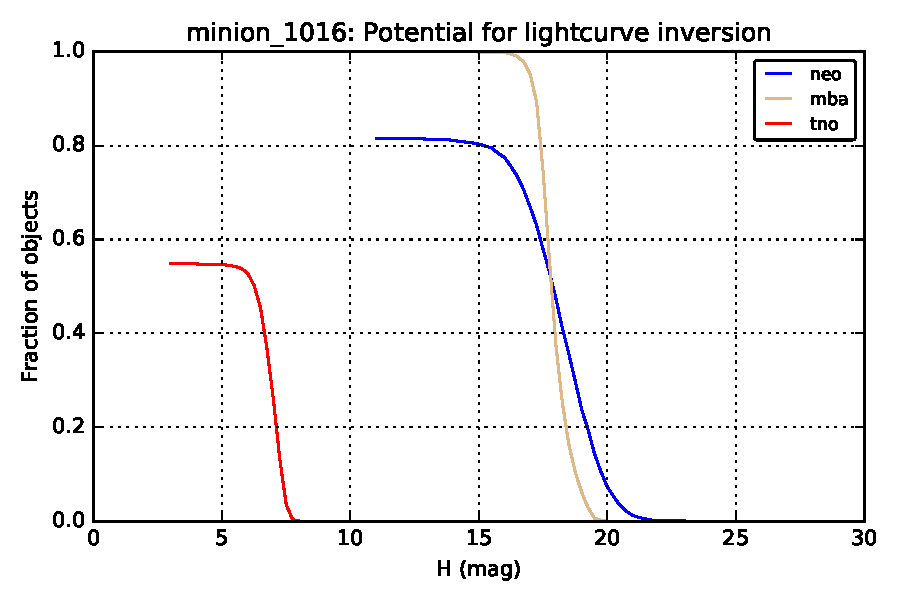
\includegraphics[width=3.3in]{figs/solarsystem/minion_1016_LightcurveInversion_neo_tno_mba_MOOB_ComboMetricVsH}
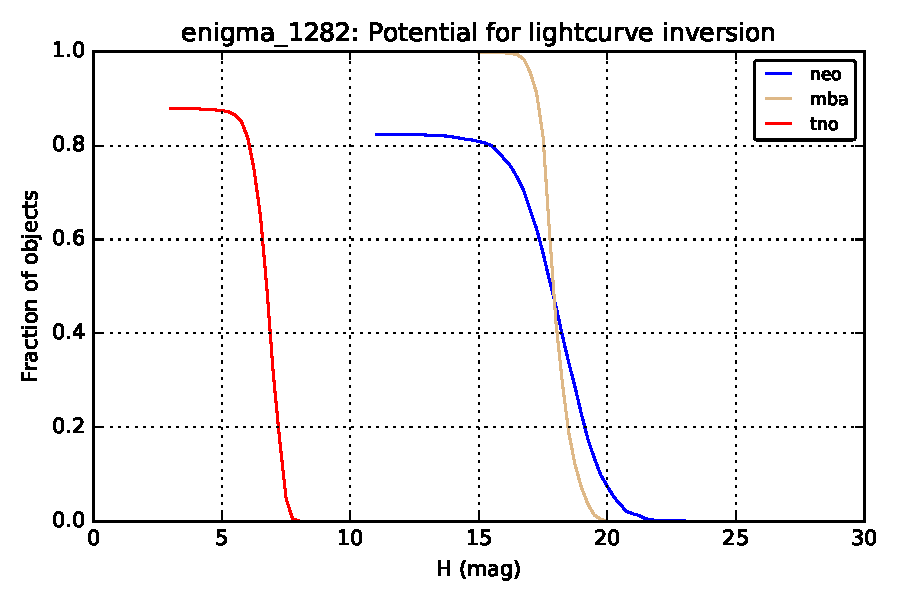
\includegraphics[width=3.3in]{figs/solarsystem/enigma_1282_LightcurveInversion_neo_tno_mba_MOOB_ComboMetricVsH}
\caption{Fraction of the sample population with the potential for
  lightcurve inversion, as a function of $H$ magnitude for NEOs, MBAs
  and TNOs, for simulated surveys \opsimdbref{db:baseCadence} and \opsimdbref{db:NEOwithVisitQuads}.
\label{lightcurveinversion}}
\end{figure}

Most solar system objects receive many observations, and bright
objects will have high SNR in most of those observations, so it is not
surprising that the baseline cadence, \opsimdbref{db:baseCadence},
performs reasonably well with this metric. Running the same metric on
other simulated surveys tends to show similar results, although
\opsimdbref{db:NEOwithVisitQuads} demonstrates that a higher fraction
of NEOs get suitable observations for lightcurve inversion. This is
illustrated in Figure~\ref{lightcurveinversion}. More
sophisticated metrics or investigation will be required to discover
the cause of this, although it seems likely that with visit quads,
there are just more observations of the bright NEOs total, leading to
a higher fraction of objects available for lightcurve inversion. The
difference between these surveys suggests that it is possible to
significantly increase the numbers of NEOs for which we can determine
shapes, rotation rates, and spin positions.

% --------------------------------------------------------------------

\subsection{Discussion}
\label{sec:\secname:discussion}

A risk which is not captured by this simple metric is that the
observations included for the lightcurve inversion estimate here,
could potentially occur far apart in time such that linking between
the observations (to determine that they belong to the same object) is
not possible.

Further work needs to be done to understand the necessary final figure
of merit, in particular, how many light curve inversion targets are
necessary, and how should they be spread among different sizes of
objects? Small objects have different shape and
rotation distributions than larger objects, so it is interesting
scientifically to understand objects at a range of $H$ magnitude. In
addition, this metric currently uses observations in any filter;
further work should be done to determine if this is sufficient, or if
observations must occur in a single filter.

% ====================================================================
%
% \subsection{Conclusions}
%
% Here we answer the ten questions posed in
% \autoref{sec:intro:evaluation:caseConclusions}:
%
% \begin{description}
%
% \item[Q1:] {\it Does the science case place any constraints on the
% tradeoff between the sky coverage and coadded depth? For example, should
% the sky coverage be maximized (to $\sim$30,000 deg$^2$, as e.g., in
% Pan-STARRS) or the number of detected galaxies (the current baseline but
% with 18,000 deg$^2$)?}
%
% \item[A1:] ...
%
% \item[Q2:] {\it Does the science case place any constraints on the
% tradeoff between uniformity of sampling and frequency of  sampling? For
% example, a rolling cadence can provide enhanced sample rates over a part
% of the survey or the entire survey for a designated time at the cost of
% reduced sample rate the rest of the time (while maintaining the nominal
% total visit counts).}
%
% \item[A2:] ...
%
% \item[Q3:] {\it Does the science case place any constraints on the
% tradeoff between the single-visit depth and the number of visits
% (especially in the $u$-band where longer exposures would minimize the
% impact of the readout noise)?}
%
% \item[A3:] ...
%
% \item[Q4:] {\it Does the science case place any constraints on the
% Galactic plane coverage (spatial coverage, temporal sampling, visits per
% band)?}
%
% \item[A4:] ...
%
% \item[Q5:] {\it Does the science case place any constraints on the
% fraction of observing time allocated to each band?}
%
% \item[A5:] ...
%
% \item[Q6:] {\it Does the science case place any constraints on the
% cadence for deep drilling fields?}
%
% \item[A6:] ...
%
% \item[Q7:] {\it Assuming two visits per night, would the science case
% benefit if they are obtained in the same band or not?}
%
% \item[A7:] ...
%
% \item[Q8:] {\it Will the case science benefit from a special cadence
% prescription during commissioning or early in the survey, such as:
% acquiring a full 10-year count of visits for a small area (either in all
% the bands or in a  selected set); a greatly enhanced cadence for a small
% area?}
%
% \item[A8:] ...
%
% \item[Q9:] {\it Does the science case place any constraints on the
% sampling of observing conditions (e.g., seeing, dark sky, airmass),
% possibly as a function of band, etc.?}
%
% \item[A9:] ...
%
% \item[Q10:] {\it Does the case have science drivers that would require
% real-time exposure time optimization to obtain nearly constant
% single-visit limiting depth?}
%
% \item[A10:] ...
%
% \end{description}
% --------------------------------------------------------------------

\navigationbar
